\documentclass[twoside,12pt]{article}
\usepackage{czech}
\usepackage[utf8]{inputenc}
\usepackage {graphicx}
\usepackage{dip}
\usepackage{amsmath}
\newcommand{\podpodsekce}[1]{\paragraph{#1}\quad\vskip 6pt}

\begin{document}
\pagestyle{headings}
\cislovat{3}
\titul{Použití laserového ukazovátka k ovládání počítače}{Tomáš Pokorný}{Mgr. Marek Blaha}{Brno 2011}

\podekovani{Na tomto místě bych chtěl poděkovat hlavně Tomáši Gavenčiakovi, který na M\&M vymyslel konferu na zpracování obrazu a jehož rady byly velmi cenné hlavně v začátcích, Karlu Královi a Lukáši Langerovi za vymyšlení poměrové transformace, Lukáši Langerovi navíc i za vymyšlení dvoubodové transformace, Janu Olšinovi za pomoc při zprovozňování projektivní transformace, Mgr. Marku Blahovi za technické zázemí a podporu při pokračování projektu a všem dalším, kteří mne svými radami nasměrovali na správnou cestu.}


\prohlaseni{Prohlašuji, že jsem tuto závěrečnou maturitní práci vyřešil samostatně s použitím literatury, kterou uvádím v seznamu.}{V Brně dne \today}
\abstract{Tomáš, P. Using a laser pointer to control a computer. Final maturita thesis. Brno, 2011}{The goal of this project is to allow user to interactively point on objects on screen using laser pointer. The screen is captured by webcam and the program is written for Mac OS X in Objective C. Application has following functions: calibration webcam, capturing an image, analysis and finding the lighted point, transformation the coordinates of found point nad final visualisation as simple drawing or game.}

\abstrakt{Tomáš, P. Použití laserového ukazovátka k obvládání počítače. Závěrečná maturitní práce. Brno, 2011}{Projekt {\it Použití laserového ukazovátka k ovládání počítače} si klade za cíl pomocí kamery a projektoru připojeného k  počítači umožnit uživateli, aby mohl využívat laserového ukazovátka jako ukazatele na objekty zobrazené projektorem na plátně. Aplikace je napsána v Objective C. Funkce aplikace jsou tyto: kalibrace webkamery pro dané umístění, zachycení a načtení obrazu z webkamery, analýza a hledání nasvíceného bodu, transformace snímaného obrazu pomocí transformační funkce a kalibračních dat a finální vykreslení vizualizace výsledků pomocí jednoduchého kreslení či hry.}

\obsah

\kapitola{Úvod a cíl práce}

!!! Jak to je teď a co jsem s tím udělal. !!!
%\sekce{Úvod do problematiky}
%Zpracování obrazu je velmi obsáhlá oblast, která zahrnuje mnoho různých oborů a problémů. Já jsem si vybral oblast hledání bodu o dané barvě v obrazu z kamery a další práce s ním. Toto v sobě zahrnuje několik kroků. Nejprve je třeba získat obraz z kamery, následně v něm najít bod\dots\footnote{A tady právě nevím, co bych tam moc napsal, protože se tím zabývám dále v sekci Popis softwaru.}
%\sekce{Cíl práce}
%Cílem práce bylo vytvořit program, který pomocí webkamery zachytává polohu laserového ukazovátka na plátně dataprojektoru a převádí ji na souřadnice, podle kterrých vykresluje na plátno počítač. Součástí práce také měly být ukázky možného využití.

\sekce{Historie projektu}
K myšlence použití laserového ukazovátka k ovládání počítače mne přivedla konfera na semináři M\&M, ve které jsme se s pomocí webkamery snažili zachytávat polohu laserového ukazovátka a ukazovat ji na projektoru. Tato konfera mne velmi zaujala a rozhodl jsem se pokračovat v ní a dovést práci dále, než se nám za krátký čas na soustředění povedlo.\footnote{Mám se tu trochu více rozepsat o tom, jak se projekt dále vyvíjel?}

\kapitola{Současný stav řešené problematiky}
Ohledně zpracování obrazu je na webu prací poměrně mnoho, avšak nenašel jsem mnoho prací, které by využívaly zpracovaný obraz k ovládání počítače (autonomní roboty pomiňme, jedná se o diametrálně odlišnou problematiku). Projektem nejbližším mé tematice je L.A.S.E.R. Tag od Graffiti Research Lab\footnote{http://graffitiresearchlab.com/projects/laser-tag/}, který se zabývá podobným cílem, avšak nemá automatickou kalibraci a bohužel se mi tento program nepodařilo zkompilovat. Dalším podobným projektem je PySight SprayPaint\footnote{http://killertux.org/projects/pysight-spraypaint}, na který jsem ale přišel až když už byla aplikace hotová. Tento program využívá Pythonovskou knihovnu PySight a neprovádí žádnou transformaci souřadnic, tudíž je poměrně nepřesný. Posledním programem, který jsem našel a zabývá se podobnou tématikou byl program, kdy laserové ukazovátko bylo použito k ovládání hry, ale tuto hru se mi bohužel nepodařilo znovu najít. Všechny tyto programy mi sloužily jako inspirace, bohužel se mi nepodařilo v jejich zdrojovém kódu nalézt části, které by mi pomohly při řešení mých problémů. 

Z hlediska mé práce nejvýznamější je framework CocoaSequenceGrabber\footnote{http://www.skyfell.org/cocoasequencegrabber.html}, který slouží pro zachytávání obrazu z integrované kamery iSight. Tento framework je v mé práci použit právě za tímto účelem.

\kapitola{Materiál a metody}
\sekce{Hardware}
Abychom mohli používat laserové ukazovátko na ovládání počítače, potřebujeme následující hardware:
\begin{itemize}
 \item{\bf Počítač} Aplikace je napsána pro Mac OS X, tudíž potřebujeme Mac s dostatečným výkonem (alespoň 1.8 GHz), aplikace je testována v Mac OS X 10.6, ale nevyužívá žádné speciality této verze systému, tudíž by měla být spustitelná i pod 10.5 a 10.4. Dále je nutné mít na počítači nainstalovaný framework CocoaSequenceGrabber
 \item{\bf Webkamera} Vzhledem k použití frameworku CocoaSequenceGrabber je použitá integrovaná kamera iSight, avšak mělo by být možné i použití externí kamery. 
\item{\bf Projektor} Na projektor nejsou kladeny žádné speciální nároky, rozlišení je potřeba nastavit na 800x600.
\item{\bf Laserové ukazovátko} Laserové ukazovátko může být jakékoli červené barvy, v případě jiné barvy je potřeba změnit barevnou složku, na kterou se bere ohled, ve zdrojovém kódu.
\end{itemize}

\sekce{Popis softwaru}
Obraz je snímán pomocí frameworku CocoaSequenceGrabber v programu HledaniBodu. Program snímá obrázky tak, jak jsou poskytovány kamerou a hledá v nich nasvícený bod. Při zpracování je vždy obraz převeden na pole bytů, nad kterým se pak provádí jednotlivé metody hledání nasvíceného bodu. Nalezené souřadnice jsou poté poskytnuty jednotlivým metodám transformace a transformované souřadnice jsou poté vizualizovány na plátně pomocí některé ze zobrazovacích tříd.

\podsekce{Metody hledání nasvíceného bodu}
\podpodsekce{Čtvercová metoda}

V této metodě se vždy počítá součet plochy 5x5 pixelů okolo zkoumaného bodu po jednotlivých barevných složkách. Před tímto výpočtem mohou být nastaveny omezující podmínky, kdy je zbytečné výpočet provádět, protože jsou body příliš tmavé, než aby na ně bylo svíceno. 

Z jednotlivých blokových součtů je zjištěno maximum hodnoty součtu hledané barevné složky a definitivně je vybrán ten bod, který má tento součet nejvyšší. U tohoto maxima jsou ještě kontrolovány součty jednotlivých složek, aby se omezily artefakty kdy pokud na projektor nesvítím se nezachytávaly zobrazené křížky.

Tato metoda se ukázala být poměrně spolehlivá, ale je potřeba najít vhodné nastavení konstant pro zahazování bodů, protože obzvláště při denním osvětlení či osvětlení různými zdroji světla  jsou snímané body různých barev a je potřeba co nejvíce špatných zahodit, ale nezahodit s nimi i ty, co chceme najít.

\podpodsekce{Křížová metoda}

Tato metoda je zjednodušenou verzí metody, o níž jsem dlouho uvažoval, ale je implementačně náročná. Metoda je založena na faktu, že hledáme bod, tzn. nějaké malé osvícené kolečko, kde má střed a několik bodů v okolí výrazně jiné vlastnosti než zbytek obrázku. Ideální stav je hledat 2 mezikruží, což je ale poměrně obtížné a tak jsem v této metodě použil jen výrazně zjednodušenou verzi.

\begin{figure}[ht]
 \begin{center}
   \scalebox{1}{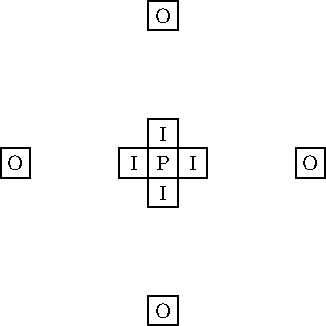
\includegraphics{kriz-1.pdf}}  
 \end{center}
 \caption{Pixely používané při křížové metodě hledání bodu.}
\end{figure}

V této verzi jsou sledovány pouze barvy aktuálně zkoumaného bodu $P$, jeho nejbližších sousedů $I$ a poté čtyř bodů $O$ vzdálených 5 pixelů na každou ze čtyř stran od bodu $P$. Pokud zrovna svítím na bod $P$, pak body $I$ budou díky své blízkosti také osvíceny poměrně výrazně a naopak na body $O$ nebude mít již nasvícení bodu $P$ žádný vliv a budou tedy reprezentovat barvu pozadí. U bodů $I$ a $O$ se počítá vždy průměr jednotlivých barevných složek ze všech 4 bodů. 

U každé skupiny bodů je možné nastavovat maximální a minimální hodnoty jasu jednotlivých složek, což dává poměrně silný nástroj k odfiltrování nežádoucích bodů. Tato metoda se ukázala spolehlivější než čtvercová, protože dokáže odfiltrovat velké jasné plochy.

\podsekce{Kalibrace}
Kalibrace je prvním z dějů souvisejících s transformací. Cílem kalibrace je zjistit, v jakých bodech na snímaném obraze se zobrazují rohy obrazu zobrazovaného dataprojektorem. To je důležité proto, abychom dokázali přepočítat bod nalezený na obrazu webkamery na bod, který zobrazíme na projektoru. Nyní k funkci kalibrace. Program postupně rozsvítí 4 čtverečky v rozích obrazu projektoru a vždy chvíli počká, aby se kamera přizpůsobila. Pak je sejme již popsaným způsobem a najde je. Tímto získáváme 4 kalibrační body, se kterými již můžeme počítat v transformacích.

\podsekce{Transformace}
\begin{figure}[ht]
 \begin{center}
   \scalebox{.75}{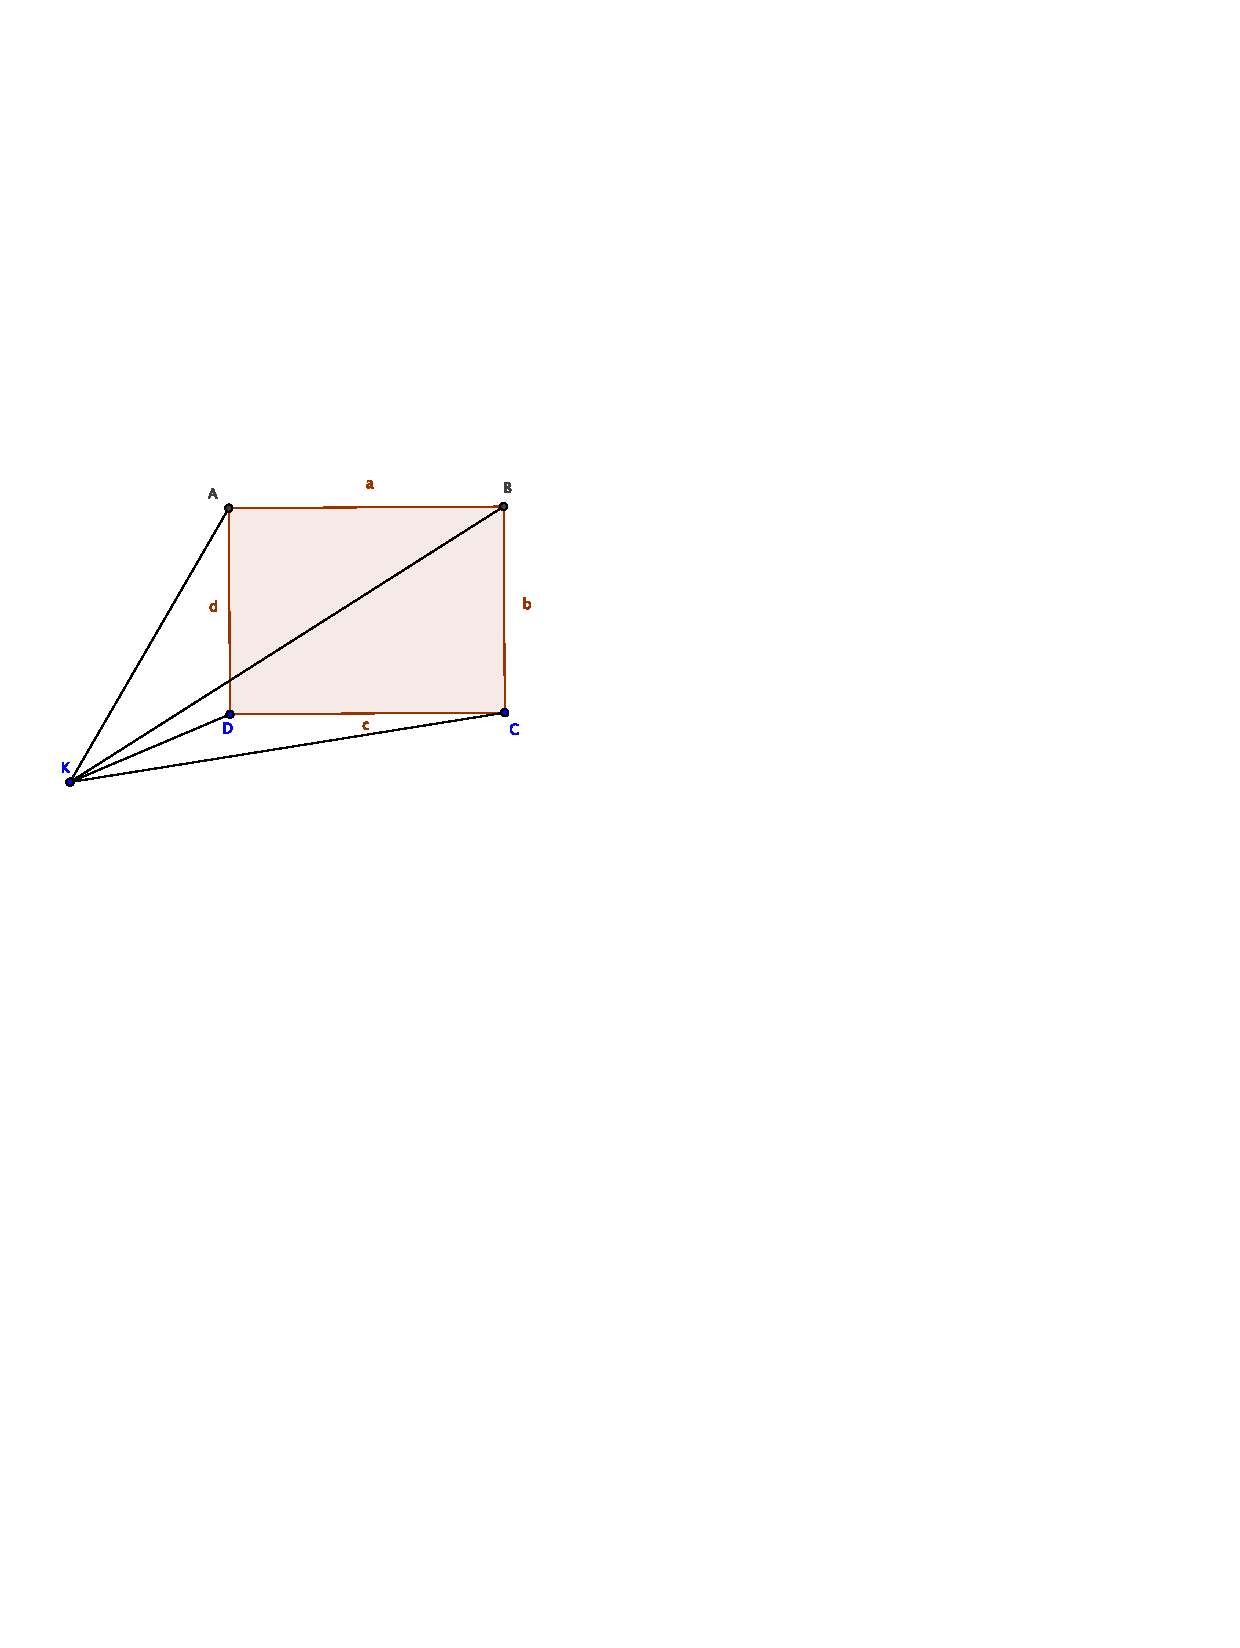
\includegraphics{../transforms/3DSituace-3D.pdf}}  
 \end{center}
 \caption{Snímání obdélníku $ABCD$ kamerou $K$ mimo osu}
\end{figure}
Toto je nejdůležitější a matematicky nejobtížnější část celého projektu, která zajišťuje správné zobrazení bodu na projektoru. Co to je a proč je potřeba?

Předpokládejme, že máme projektor, který promítá na plátno obdélníkový obraz. Pokud by ho promítal zkreslený, má své vlastní funkce ke korekci tohoto zkreslení. Pokud nyní obraz snímáme kamerou, získáme nějaký útvar. Optimální situace nastává, pokud kamera snímá ze stejného bodu, jako promítá projektor. V tom případě je snímaný útvar obdélník se stejným poměrem stran k promítanému obrazu. Tady nám stačí úplně základní transformace a to jednoduché přinásobení konstantou odpovídající poměru délky strany snímaného a promítaného obrazu. Toto je ale situace, která nastane velmi zřídka. Většinou snímáme kamerou obraz zkreslený, protože pokud si představíme to, co snímá kamera, jde o jakýsi nekonečně vysoký čtyřboký jehlan.
\begin{figure}[ht]
 \begin{center}
   \scalebox{.75}{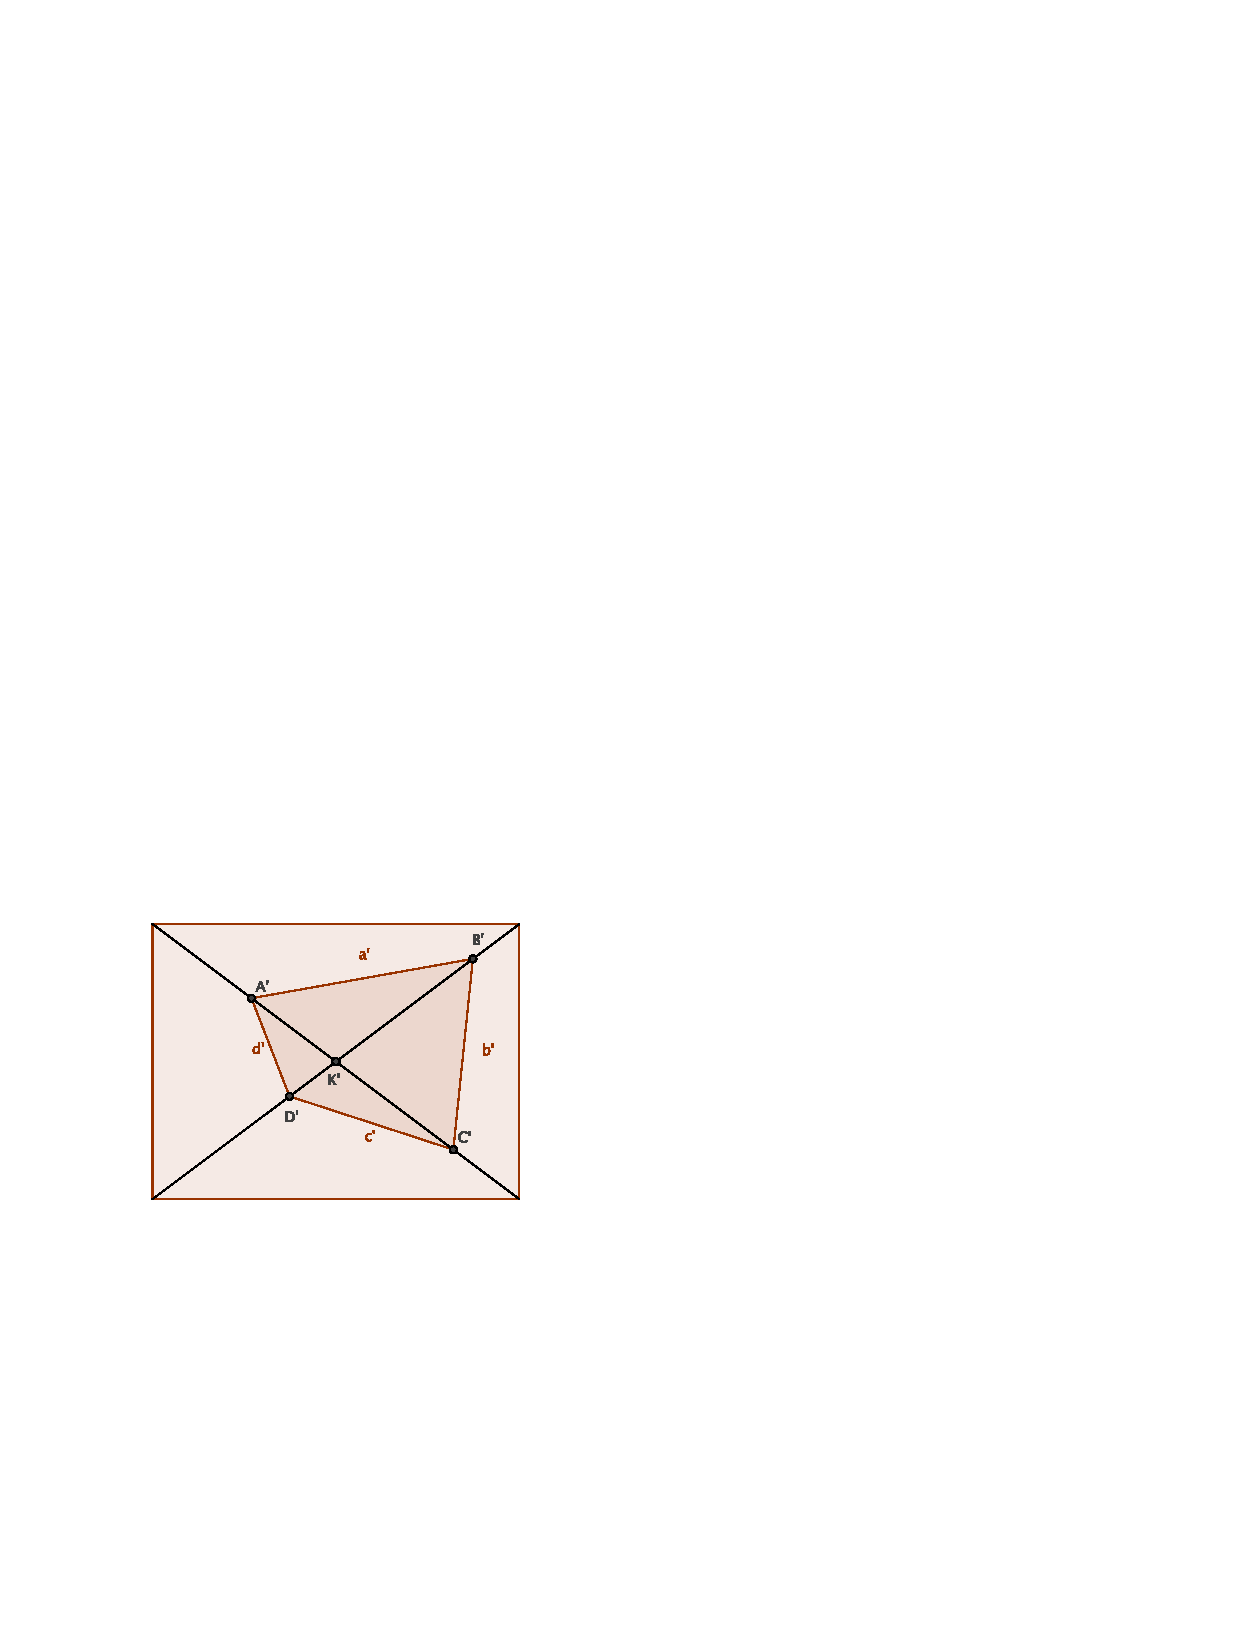
\includegraphics{../transforms/3DSituace-2D.pdf}}  
 \end{center}
 \caption{Zkreslený útvar $A'B'C'D'$ tak, jak ho vidí kamera}
\end{figure}

Pokud snímáme útvar mimo osu projektoru, bude snímaný útvar určitým řezem daného jehlanu, tudíž to bude docela obecný čtyřúhelník. My potřebujeme tento čtyřúhelník roztáhnout vhodně tak, abychom získali obdélník, který bude odpovídat obdélníku promítanému projektorem, abychom mohli tento obdélník zobrazit. To je právě záležitost transformace.

\podpodsekce{Transformace se 2 body}

\begin{figure}[ht]
 \begin{center}
   \scalebox{.75}{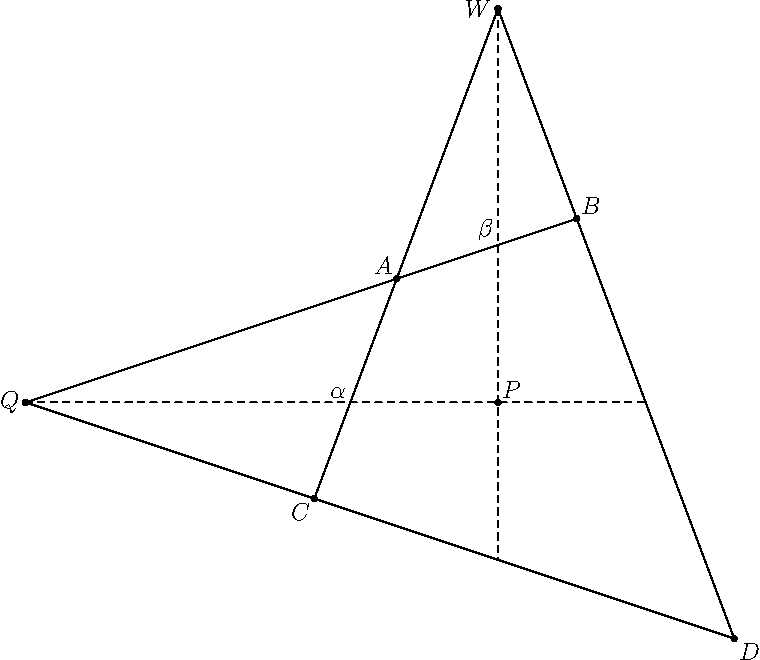
\includegraphics{2p-transform-1.pdf}}  
 \end{center}
 \caption{Schéma dvoubodové transformace}
\end{figure}
Tato transformace je vymyšlená Lukášem Langerem. Základem je to, že při zachycení zkresleného obrazu se původně rovnoběžné přímky určené rohovými body $A$, $B$, $C$ a $D$ budou sbíhat a tudíž se protnou v nějakém bodě ($Q$, $W$). Tento bod jednoduše nalezneme prodloužením stran. Přímka procházející zachyceným bodem $P$ a rovnoběžná se stranou  $AC$ nebo $AB$ na skutečném plátně bude při zkreslení procházet nalezeným průsečíkem $Q$ či $W$. Nalezneme průsečík této přímky se stranou $AB$ nebo $AC$, nazveme ho $\alpha$ a $\beta$ a určíme poměr části k průsečíku k celé této straně. Toto provedeme pro obě rovnoběžné strany a získané poměry stačí vynásobit šířkou a výškou zobrazovaného obrazu. Tato transformace dává výsledky s přesností okolo 5 cm.

\podpodsekce{ Poměrová transformace}

Základem je fakt, že i ve zkresleném útvaru zůstanou zachovány poměry vzdáleností a to speciálně poměrů vzdáleností nalezeného osvíceného bodu od stran. Pokud tuto úvahu zobecníme na dva rozměry, získáme rovnice, pomocí kterých můžeme získané souřadnice nalezeného bodu přepočíst na souřadnice bodu na obrazovce.

\podpodsekce{ Projektivní transformace}
%Reference
Princip projektivní transformace je vysvětlen v [1]. Projektivní transformace umí převádět mezi souřadnicemi v jedné a druhé rovině, což je přesně to, co potřebujeme. Transformační rovnice dopředné transformace jsou 
\begin{align*}
 x' &= \frac{a_0x+a_1y+a_2}{a_6x+a_7y+1}
 y' &= \frac{a_3x+a_4y+a_5}{a_6x+a_7y+1}
\end{align*}
Koeficienty se dají také pěkně zadat do matice:
$$\left[
 \begin{array}{c} 
  u'\\
  v'\\
  w'\\
 \end{array}
\right]
=
\left[
 \begin{array}{c}
 x\\
 y\\
 1\\
 \end{array}
\right]
\cdot
\left[
 \begin{array}{ccc}
 a_1 & a_2 & a_3\\
 a_4 & a_5 & a_7\\
 a_7 & a_8 & 1\\
 \end{array}
\right]
  $$
Vzniklý vektor musíme ještě normalizovat:
\begin{align*}
 x' &= \frac{u'}{w'}
 y' &= \frac{v'}{w'}
\end{align*}

Na vypočítání koeficientů transformace musíme naleznout inverzní matici transformace a spočítat její koeficienty. Tuto část mi pomohl udělat Jan Olšina\footnote{organizátor M\&M, jan.olsina@gmail.com} v Mathematice, za což mu přísluší velký dík. Získané koeficienty pak již stačí jen přepsat do zdrojového kódu. Tato transformace je nejpřesnější, protože jde o přesné matematické vyjádření. S touto transformací se podařilo dosáhnout přesnosti jednotek centimetrů, kde je přesnost limitována rozlišením kamery.

\podpodsekce{ Další transformace}
Během vývoje vznikly ještě 2 další transformace a to transformace přibližná, která vždy předpokládala, že útvar je lichoběžník a to postupně v obou rozměrech a výsledek pak zprůměrovala. Toto byla používaná transformace v začátcích, než byla odhalena chyba v transformaci poměrové. Se stoupajícím zkreslením rapidně klesá přesnost. 

Druhá ze vzniklých transformací byla založena na úhlech a postupném posouvání kalibračních bodů do vrcholů promítaného čtyřúhelníka. Při nasimulování její činnosti ale bylo zjištěno, že byly úvahy chybné a tato transformace nemůže fungovat.

Využívanou transformací v dobách, kdy byl projekt v Pythonu, byla transformace grafická, která využívala knihovní funkce Python Image Library, ale tuto transformaci se nepodařilo převést do Objective C.

\podsekce{Zobrazení}
Obraz se vykresluje do černého okna o velikosti obrazu promítaného projektorem. Při vykreslování je třeba dbát na to, aby barva, kterou kreslíme, nebyla příliš jasná nebo se nepodobala barvě laserového ukazovátka. V prvním případě totiž dojde k přepalům v obraze, v druhém k chybbnému vyhodnocení osvíceného bodu a oba tyto problémy vedou k nepřesnostem a chybám v zobrazování.


\kapitola{Výsledky}
Pokud známe umístění bodu vůči plátnu, tzn. jeho polohu v souřadnicích projektoru, máme mnoho možností, jak ho vizualizovat. Níže jsou popsány výsledné aplikace, které slouží jako ukázka možností projektu.

\sekce{ Kreslení jednou barvou}
% Obrázek
V tomto případě se přepočítaný bod uloží do Beziérovy křivky, která se při každém nově příchozím bodu opět vykreslí. Pokud se bod nepodaří nalézt, tak se čeká, než je nalezen nějaký platný bod a do tohoto bodu se kreslení přesune bez toho, aby kreslilo čáru. Tímto se tedy dají kreslit i přerušované čáry. Kresba se dá resetovat a dá se zvolit tloušťka čáry. Kresba se dá uložit a pomocí externího perlového skriptu bezpath2svg.pl převést na SVG soubor.

\sekce{ Kreslení třemi barvami}
\begin{figure}[ht]
 \begin{center}
   \scalebox{.5}{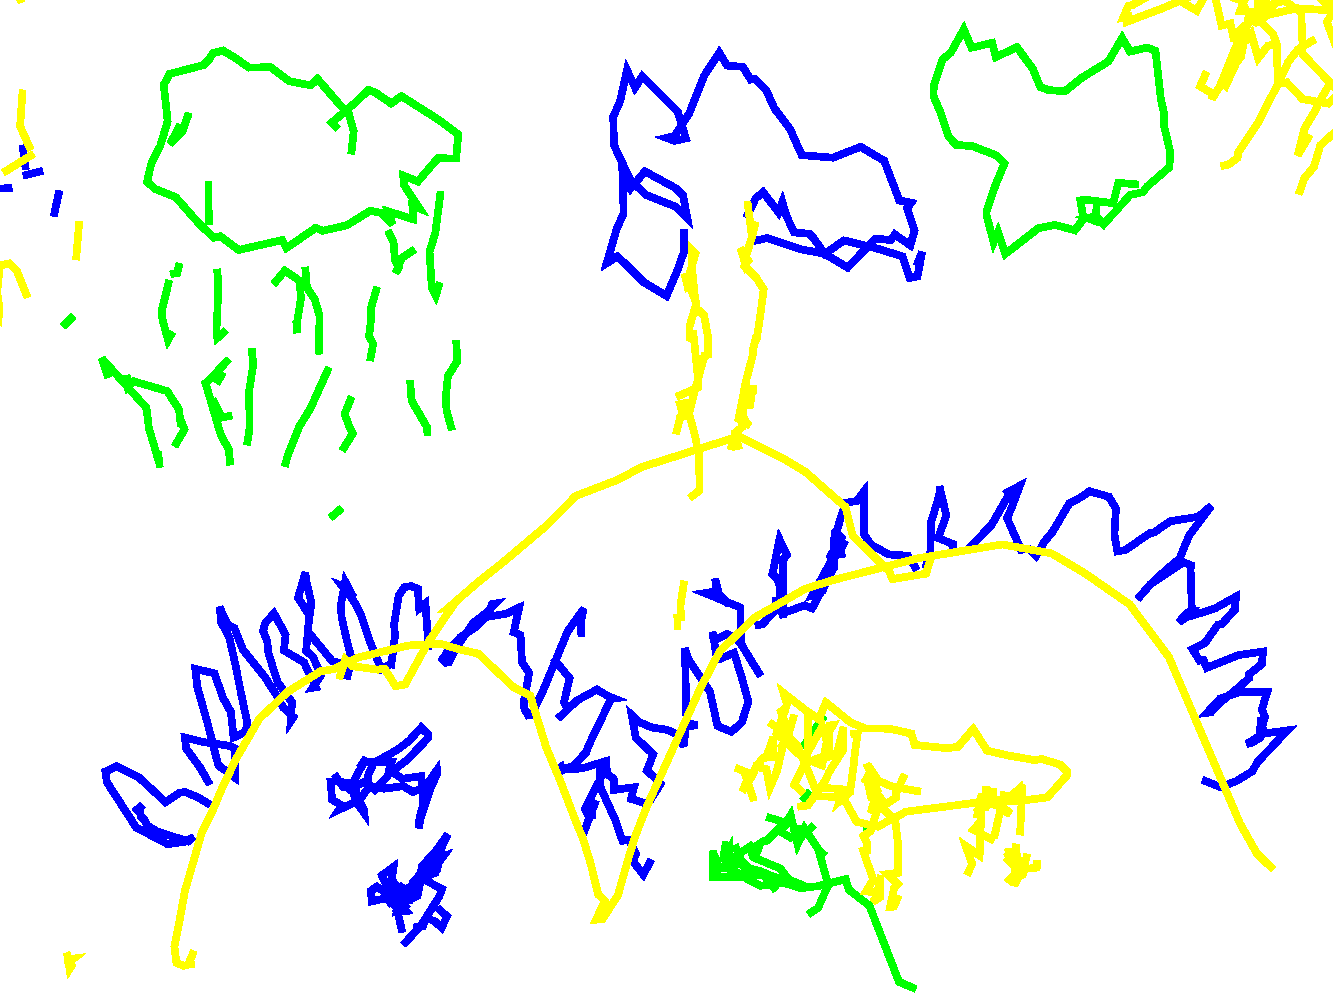
\includegraphics{../images/kopecky.pdf}}  
 \end{center}
 \caption{Ukázka možností kresby třemi barvami}
\end{figure}
Princip je stejný jako u kreslení jednou barvou, ale v tomto případě jsou Bézierovy křivky tři, pro každou barvu jedna. Přepínání mezi barvami je pomocí tří barevných čtverců v levém horním rohu obrazu promítaného projektorem. Pod těmito barvami je čtverec pozastavující kreslení a v levém dolním rohu je čtverec, na kterém když je setrváno alespoň 20 zpracovaných snímků, kresba se resetuje. Stejně jako při kreslení jednou barvou se dá kresba uložit a převést do SVG.

\sekce{Střílení balonků}
\begin{figure}[ht]
 \begin{center}
   \scalebox{.5}{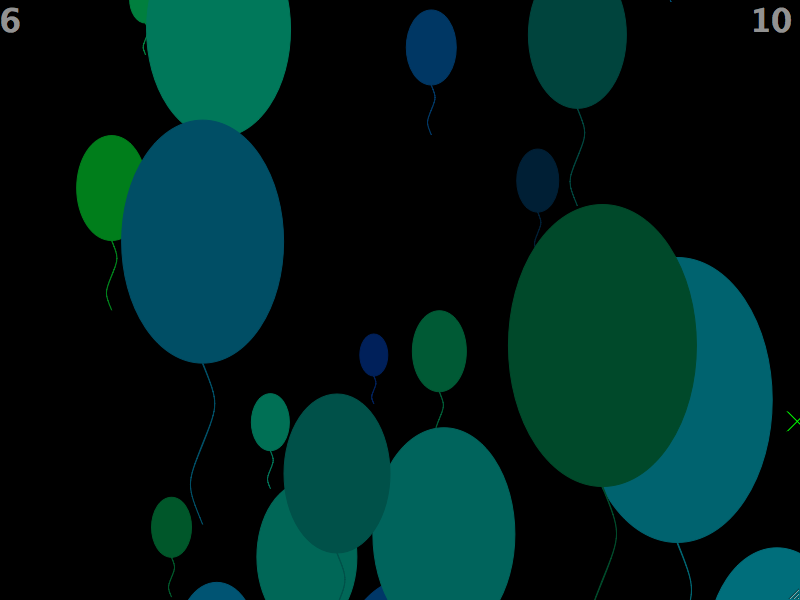
\includegraphics{../images/shooting.png}}  
 \end{center}
 \caption{Střílení balonků}
\end{figure}
Toto je ukázka, jak lze využít laserového ukazovátka pro ovládání hry. Na plátno se promítají různě velké a barevné balonky, které stoupají vzhůru a laserového ukazovátka se využívá k jejich sestřelování. Je možné si zvolit parametry hry, na obrazovce je zobrazen počet ulétlých a sestřelených balonků.

\kapitola{Diskuse}
\sekce{Srovnání s podobnými aplikacemi}
Souhrn aplikací s podobnými vlastnosti jsem již uvedl na začátku. L.A.S.E.R Tag je aplikace o mnoho větší a umožňuje velmi pokročilé činnosti, jediná výhoda mé aplikace spočívá v automatické kalibraci plátna. Oproti dalším aplikacím je největší výhodou projektivní transformace, která zajišťuje vysokou přesnost, i když kamera se nedívá na plátno kolmo.
\sekce{Problémy v průběhu práce}
Prvním, zásadním a nejhloupějším problémem byl problém s poměrovou transformací. Jeho podstata byla v odlišném číslování rohů obdélníka při kalibraci a při transformaci. Tato chyba nás zdržela o jedno odpoledne, kdy jsme mohli pokračovat v programování. Byla odhalena až asi v polovině prezentace konfery na soustředění M\&M. 

Problémy byly při přepisování do Objective C, ale byly úspěšně překonány. Největším problémem bylo vždy rozběhat danou transformaci, protože při přepisování do počítače vznikla vždy alespoň jedna chyba, která se dost těžko hledala. Tyto problémy se táhly dlouhou dobu, je to vidět i na tom, že první námi naprogramovaná transformace se podařila zprovoznit až za dlouhou dobu a například zprovoznit dvoubodovou transformaci trvalo od 27. ledna, kdy byla uveřejněna na SVN až do 18. března, kdy vyšla stabilní revize.

Dalším problémem bylo kreslení, při němž jsem si nevšiml, že [NSBezierPath bezierPath] je autorelease a divil jsem se, že do ní pak při dalším volání metody nešlo zapisovat.

Při přechodu na využívání vazeb se vyskytl problém se čtením hodnot. Sice fungovalo nastavování, ale v GUI se to nezobrazovalo. Příčina nebyla zjištěna, nyní to již funguje tak, jak má.

Nejdéle trvajícím problémem bylo zprovoznění použitelné transformace. V době ročního výročí opět na podzimním M\&M se mi s vydatnou pomocí Irigiho podařilo zprovoznit projektivní transformaci, která je matematicky správně, a přesnost je již záležitostí rozlišení kamery. 

Drobným problémem při implementaci střílení balonků bylo zjištění, že maxSize je rezervované slovo a tudíž nelze použít jako název proměnné. To bylo obejito použitím názvu maxiSize, které sice nezapadá do používaného značení, ale nekoliduje s rezervovaným slovem.

Občas se také vyskytly problémy se SVN, kdy některý commit nechtěl být přijat, ale nakonec se tyto problémy podařilo vždy vyřešit zkopírováním vhodných .svn do problémových složek.

\kapitola{Využití v praxi}
Využití pro kreslení a střílení balonků je zmíněno výše. Jako další využití se nabízí možnost náhrady interaktivní tabule pomocí laserového ukazovátka nebo svítícího pera. Pro toto použití by bylo nezbytné použít dostatečně silného světelného zdroje, aby byl odlšitelný od obrazu na plátně. Také by byla potřeba kamera bez automatické regulace jasu, protože by se dala lépe nastavit na daný zdroj světla. 

Další možností využití jsou, při použití více barev laserů, různé multiplayerové hry ukazovátky ovládané. Při vhodném pozadí a správném nastavení barev by se mohlo kreslení využívat pro zkoumání trajektorií například vržených předmětů.

\kapitola{Závěr}
V současné době je projekt plně použitelný s výše zmíněnými aplikacemi. Nyní je projekt stabilní, hledání bodu je poměrně spolehlivé, transformace přesná. Práce na projektu trvaly dlouhou dobu, během které se zlepšily některé počáteční nedostatky (např. rozdělení zdojového kódu do mnoha tříd, protokoly). Aplikace je oproti dřívějším dobám rychlejší a umožňuje pracovat s vyšším rozlišením. 

\sekce{Nápady do budoucna}
\podpodsekce{Zpracování obrazu}
\begin{itemize}
\item automatické nastavení maximálních a minimálních jasů
\item odfiltrování oblastí mimo plátno s využitím kalibračních dat
\item možnost volby rozlišení v GUI
\end{itemize}
\podpodsekce{Kalibrace}
\begin{itemize}
\item ukládání kalibračních dat
\item automatické načítání kalibračních dat při startu aplikace
\end{itemize}
\podpodsekce{Kreslení}
\begin{itemize}
\item nastavování šířky laserovým ukazovátkem
\item automatická konverze do SVG
\item možnost výběru libovolné barvy (i laserovým ukazovátkem)
\end{itemize}
\podpodsekce{Střílení balonků}
\begin{itemize}
\item zrychlení vykreslování
\item změny na balonku v závislosti na počtu zásahů
\item efektní sestřelení balonku
\item v průběhu hry postupně zrychlující balonky
\item odladit okrajové situace
\end{itemize}

\end{document}
